\chapter{Experiments and Evaluation}
\label{ch:4}
\label{sec:4}


This chapter presents the quantitative evaluation. \cref{sec:4_1} defines the experimental strategy, including dataset statistics, comparison-route families, and all evaluation metrics. \cref{sec:4_2} reports the quantitative results, while \cref{sec:4_3} presents the qualitative and diagnostic analyses. The finding statement accompanying each table describes only the observed pattern; causal interpretation is reserved for \cref{sec:5}.


\section{Strategy and Metrics}
\label{sec:4_1}


\subsection{Dataset Statistics}
\label{sec:4_1_1}


The SVI manifest described in \cref{sec:3_2_2} contains 10,104 buildings and 47,238 images. After linkage with the quality-controlled and TABULA-NL-matched building-level reference table, 88 images associated with 18 buildings are excluded from model development and evaluation because of invalid 3DBAG geometry or unsuccessful archetype matching. All experiments in this chapter therefore use the final population of \textbf{10,086 buildings and 47,150 images}, comprising 8,068 buildings in the development set and 2,018 buildings in the frozen hold-out set. The values 10,104 and 10,086 do not represent contradictory counts of the same set: the former is the SVI data-delivery scope after image curation, whereas the latter is the modelling sample with complete experimental inputs and reference targets.



\begin{table}[H]
\centering
\caption{City composition and fixed data partition of the experimental dataset}
\label{tab:4_1}
\footnotesize
\begin{tblr}{
  width = \linewidth,
  colspec = {X[1.7,l] X[1,r] X[1,r] X[1,r] X[1,r] X[1,r] X[1,r]},
  row{1} = {font=\bfseries},
  rowsep = 3pt,
  colsep = 4pt
}
\toprule
City & Dev. buildings & Dev. images & Hold-out buildings & Hold-out images & Total buildings & Total images \\
\midrule
Amsterdam & 6,416 & 29,309 & 1,595 & 7,215 & 8,011 & 36,524 \\
Rotterdam & 1,129 & 5,864 & 286 & 1,460 & 1,415 & 7,324 \\
Utrecht & 384 & 1,778 & 103 & 454 & 487 & 2,232 \\
Delft & 139 & 871 & 34 & 199 & 173 & 1,070 \\
\textbf{Total} & \textbf{8,068} & \textbf{37,822} & \textbf{2,018} & \textbf{9,328} & \textbf{10,086} & \textbf{47,150} \\
\bottomrule
\end{tblr}
\end{table}


The experimental sample is highly concentrated geographically: Amsterdam contains 8,011 buildings, corresponding to 79.4\% of the experimental dataset. Its building-type composition also differs substantially from that of the eligible four-city registry reference pool, which comprises 124,784 residential buildings with EPCs that permit TABULA-NL matching. Apartment Blocks (AB) account for approximately 88\% of the experimental sample, compared with approximately 54\% of the reference pool. The EPC-label distributions of the two sets also differ, but this difference cannot be characterised simply as a bias towards better ratings in the experimental sample. Under the binary grouping used in this study, A--C accounts for 70.3\% of the experimental sample and 76.5\% of the reference pool. Subsequent results should therefore be interpreted as estimates for this SVI-covered sample rather than unbiased estimates for the residential building stock of the four cities.


This mismatch in sample composition is consistent with the contributor-driven, non-random spatial coverage of Mapillary and is also influenced by the study area, residential-eligibility criteria, and image-quality screening. The observed bias is not further attributed to specific contributor behaviour. The effect of pool composition on model performance is measured in \cref{sec:4_3_5}, and the resulting limitation on the scope of the study is discussed in \cref{sec:5_2}.


\begin{figure}[htbp]
\centering
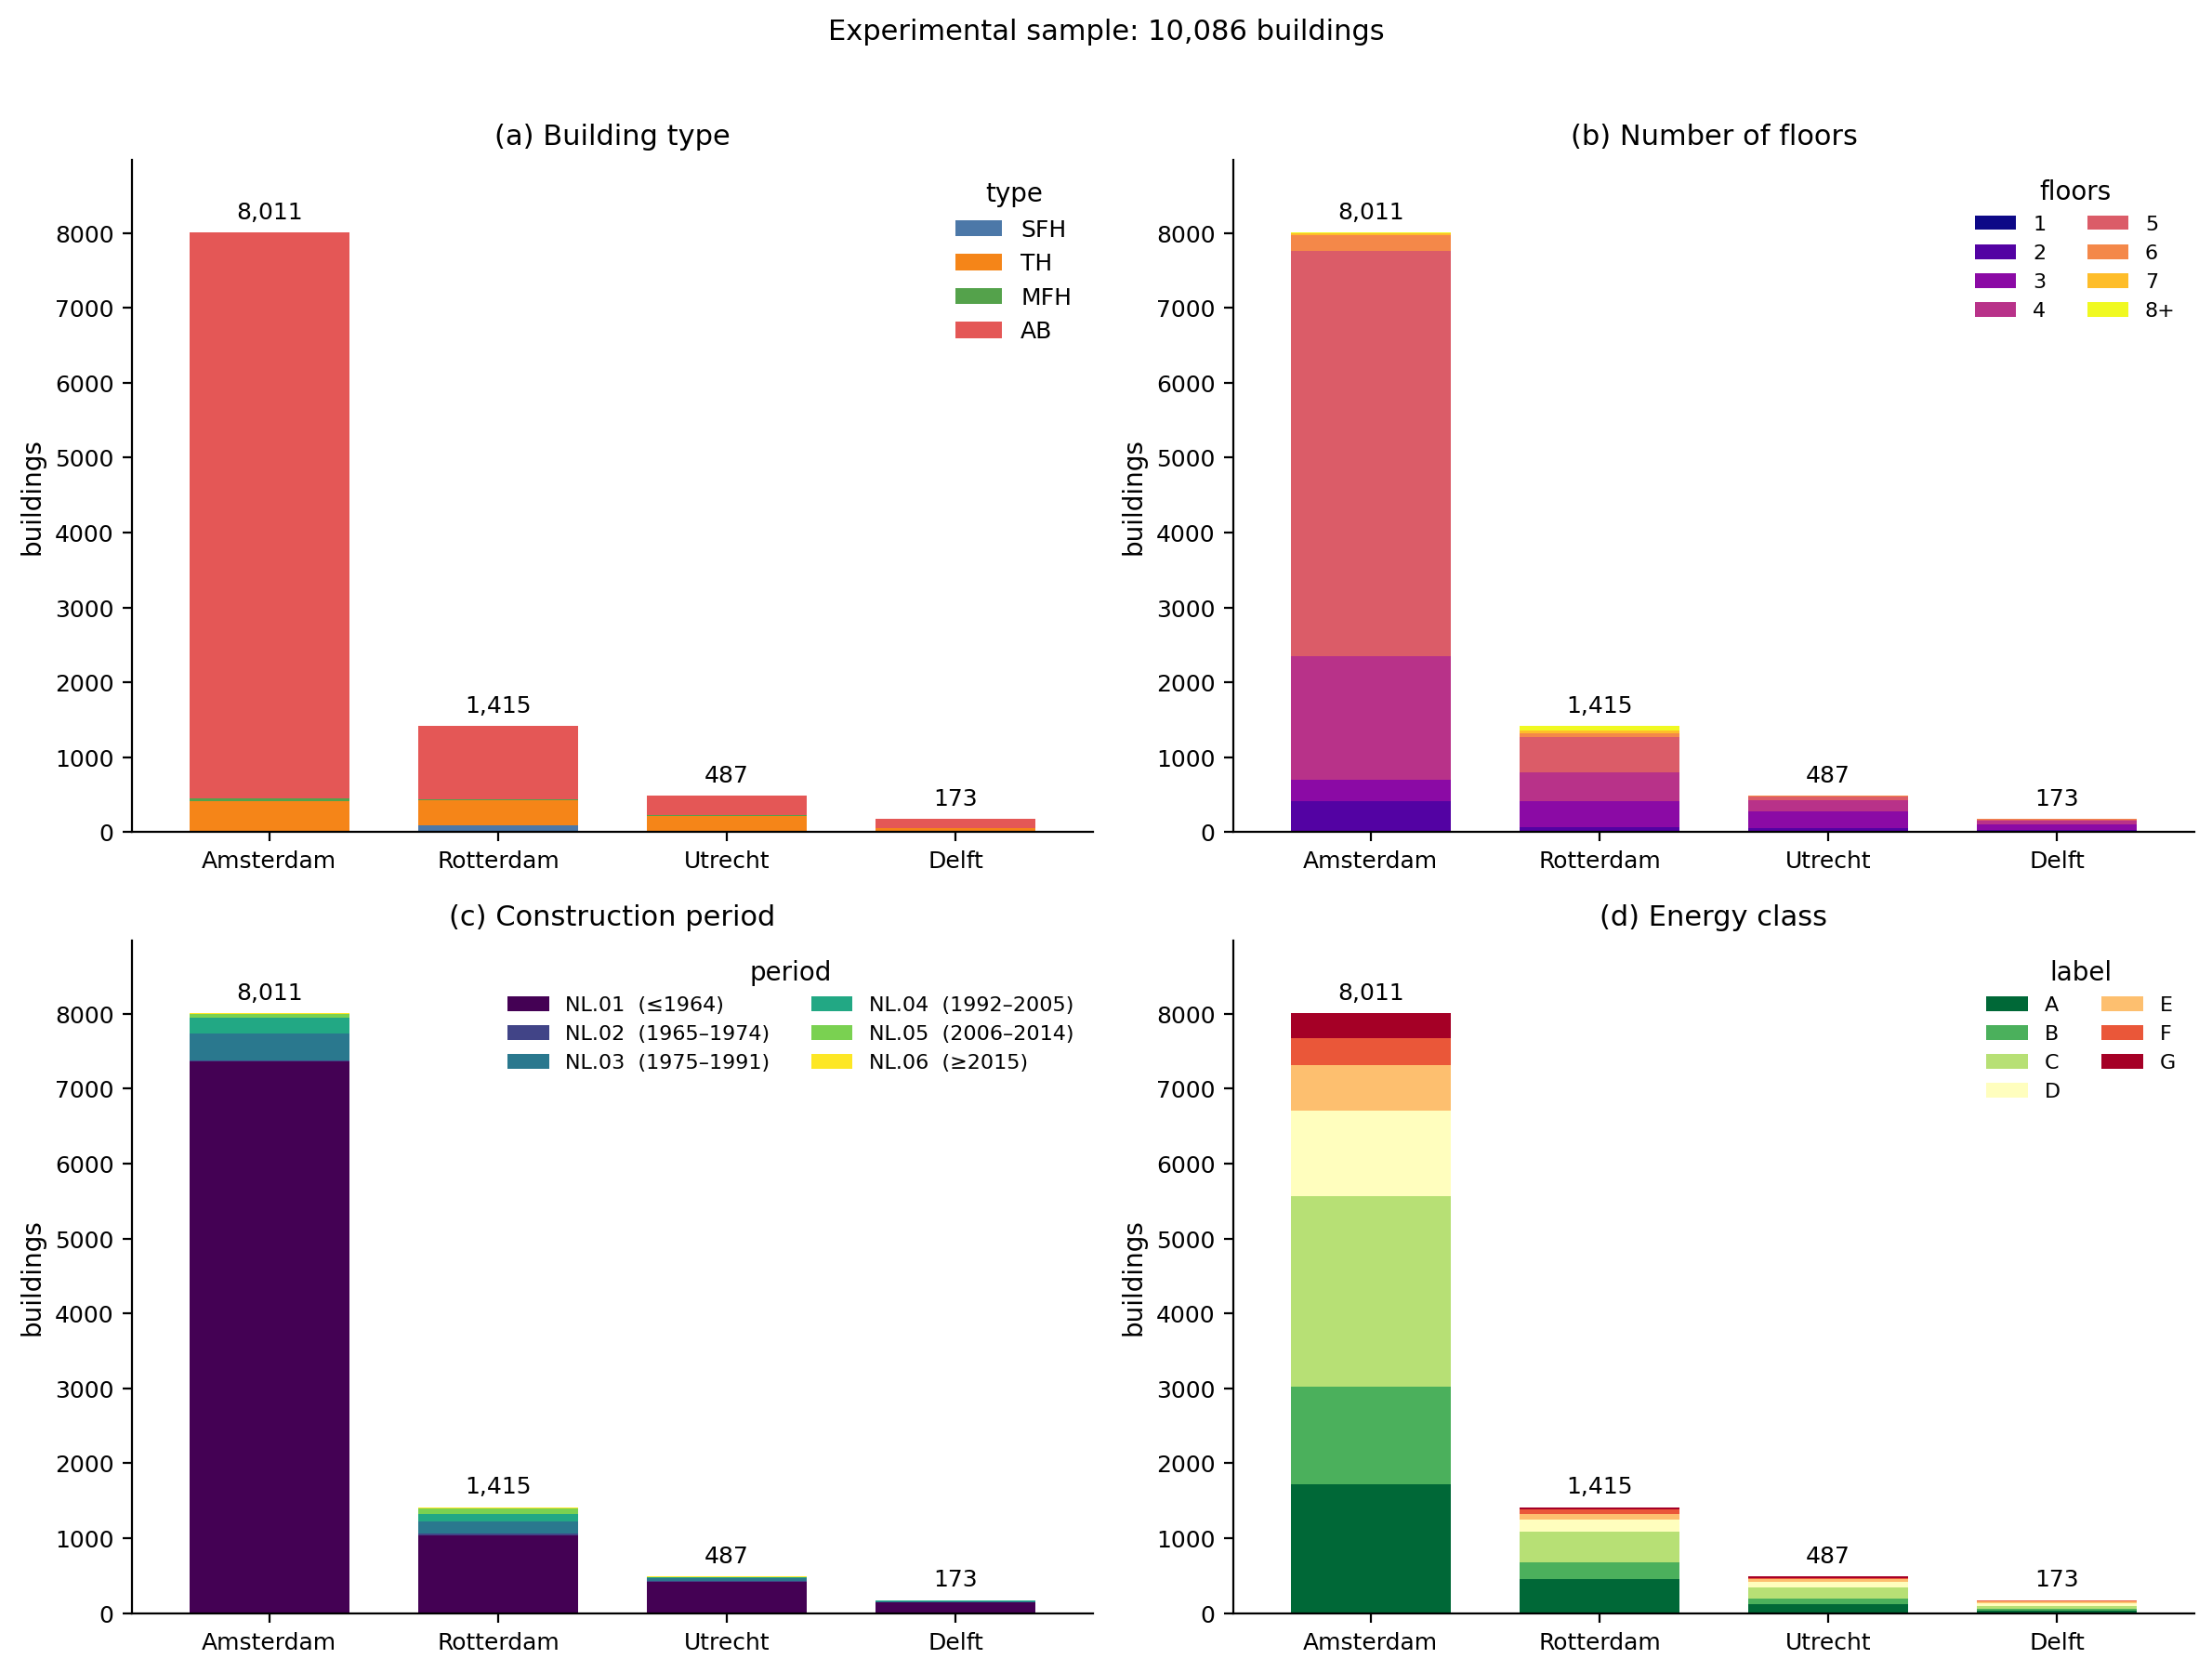
\includegraphics[width=0.98\linewidth,height=0.70\textheight,keepaspectratio]{figures/fig/fig_4_1_distributions.png}
\caption{Experimental-sample attribute and EPC-label distributions by city.}
\label{fig:4_1}
\end{figure}


\subsection{Route Families and Evaluation Settings}
\label{sec:4_1_2}


\textbf{Route families.} Four evaluation routes distinguish a no-information baseline, reference-attribute inference, direct prediction from imagery, and attribute-mediated inference. The M identifiers denote inference routes rather than different datasets or downstream-model families.


\begin{table}[H]
\centering
\small
\begin{tblr}{
  width = \linewidth,
  colspec = {X[1.7,l] X[1,l] X[1,l] X[1,l]},
  row{1} = {font=\bfseries},
  rowsep = 3pt,
  colsep = 4pt
}
\toprule
Route & Input attributes & Inference procedure & Role in the comparison \\
\midrule
\textbf{M0} & No building attributes or image input & Output the majority class of the corresponding development training data for all evaluation buildings & No-information baseline \\
\textbf{M1} & Reference building type, construction year, floor count, four U-values obtained from the reference TABULA-NL cell, and city & Input the eight reference-derived features to the fixed LightGBM EPC classifier & Reference-attribute baseline \\
\textbf{M2} & Street-view images & Predict the binary or seven-class EPC label directly from imagery without attribute prediction, TABULA lookup, or LightGBM & End-to-end comparator \\
\textbf{M3} & Vision-predicted building type, construction year, floor count, four U-values obtained from the predicted TABULA-NL cell, and city & Input the eight vision-derived features to the same fixed LightGBM EPC classifier used for M1 & Attribute-mediated route \\
\bottomrule
\end{tblr}
\end{table}


\textbf{Evaluation settings (WIP).} The primary evaluation uses the fixed building-level split defined in \cref{sec:3_2_3}: 8,068 development buildings and a frozen hold-out set of 2,018 buildings. The five development folds support model selection and OOF analyses, whereas all pooled headline results are reported on the untouched hold-out set. A separate Amsterdam-held-out transfer test trains and selects all trainable components using 2,075 buildings from Rotterdam, Utrecht, and Delft and evaluates them on 8,011 Amsterdam buildings. The original pooled split is not retained in this setting. Because Amsterdam is the only held-out city, this experiment identifies a city-shift boundary rather than estimating average cross-city generalisation.


\begin{quote}
WIP summary. The ResNet-50, DINOv2, and InternVL3-2B configurations retain the parameter-update scopes, image counts, and multi-image aggregation procedures defined in \cref{sec:3_3} and \cref{tab:3_3}. Each configuration produces an M3 attribute-mediated variant and a separately configured M2 direct-EPC comparator.
\end{quote}


\subsection{Prediction Tasks and Metrics (WIP)}
\label{sec:4_1_3}


\begin{quote}
WIP summary. Upstream evaluation covers building-type accuracy and macro-F1, construction-year MAE and TABULA-period accuracy, and floor-count MAE. Archetype assignment is assessed using joint-cell accuracy, a majority-cell baseline, and macro-cell recall. Binary A--C/D--G classification is the primary downstream task and uses ROC-AUC as its principal threshold-independent metric, with macro-F1 reported at the default and rate-matched operating points. Seven-class A--G prediction is retained as a diagnostic task using macro-F1, quadratic weighted kappa, exact and \ensuremath{\pm}1 accuracy, and class-distance MAE. Error attribution separates cases in which upstream attributes are correct but downstream classification fails from cases involving upstream attribute errors.
\end{quote}


\subsection{Physical-Consequence Metric (WIP)}
\label{sec:4_1_4}


\begin{quote}
WIP summary. The planned physical-consequence analysis reweights archetype-cell errors through the transmission heat-transfer coefficient \(H'_{tr}\), calculated from predicted TABULA U-values and reconstructed 3DBAG envelope areas. It will report building-level error and floor-area-weighted stock-level heat-loss bias under a window-to-wall-ratio sensitivity analysis. This metric compares predicted and reference archetype cells; it is not a validation against measured energy consumption.
\end{quote}


\section{Quantitative Results}
\label{sec:4_2}


\subsection{Upstream Attribute Extraction}
\label{sec:4_2_1}


\Cref{tab:4_2} compares the three vision configurations on the frozen hold-out set. Building type is evaluated using accuracy and macro-F1, construction year using MAE and TABULA-NL period accuracy, and floor count using MAE.



\begin{table}[H]
\centering
\caption{Upstream attribute extraction on the hold-out set (\(n = 2{,}018\))}
\label{tab:4_2}
\footnotesize
\begin{tblr}{
  width = \linewidth,
  colspec = {X[1.7,l] X[1,r] X[1,r] X[1,r] X[1,r] X[1,r]},
  row{1} = {font=\bfseries},
  rowsep = 3pt,
  colsep = 4pt
}
\toprule
Vision configuration & Type accuracy & Type macro-F1 & Year MAE (years) & Period accuracy & Floor MAE \\
\midrule
DINOv2, frozen backbone & 0.901 & \textbf{0.520} & \textbf{9.45} & \textbf{0.901} & \textbf{0.377} \\
ResNet-50, full fine-tuning & \textbf{0.915} & 0.492 & 11.82 & 0.892 & 0.428 \\
InternVL3-2B, zero-shot & 0.495 & 0.246 & 30.65 & 0.769 & 0.708 \\
\bottomrule
\end{tblr}
\end{table}


ResNet-50 achieved the highest building-type accuracy, whereas DINOv2 obtained the highest type macro-F1 and the lowest errors for construction year and floor count. The difference between accuracy and macro-F1 indicates that aggregate type accuracy was strongly influenced by the dominant Apartment Block class; macro-F1 provides the more informative assessment of performance across the four building types. DINOv2 therefore provided the strongest overall balance across the three extracted attributes, although ResNet-50 retained a small advantage in type accuracy. InternVL3-2B performed substantially below both trained configurations on every reported metric. This result characterises the specific open-source 2B zero-shot configuration evaluated here and should not be interpreted as a general limitation of all zero-shot vision-language models.


\subsection{Joint-Cell Assignment}
\label{sec:4_2_2}


DINOv2 and ResNet-50 achieved nearly identical joint-cell accuracies of 0.825 and 0.826, respectively, only approximately 3.5 percentage points above the majority-cell baseline of 0.790. DINOv2 obtained the higher macro-cell recall, but its performance remained strongly concentrated in the dominant cells: recall was 0.932 for AB | NL.01 and 0.789 for TH | NL.01, compared with 0.247 for AB | NL.03 and 0.074 for AB | NL.04. InternVL3-2B did not exceed the majority-cell baseline. These results show that high aggregate type and period accuracy did not translate into broad coverage of the TABULA-NL matrix; the trained configurations primarily provided reliable assignment for the cells most frequently represented in the hold-out set.



\begin{table}[H]
\centering
\caption{Joint-cell assignment on the hold-out set (majority-cell baseline = 0.790)}
\label{tab:4_3}
\small
\begin{tblr}{
  width = \linewidth,
  colspec = {X[1,l] X[1,r] X[1,r]},
  row{1} = {font=\bfseries},
  rowsep = 3pt,
  colsep = 4pt
}
\toprule
Paradigm & Joint accuracy & Macro-cell recall \\
\midrule
DINOv2 (frozen) & 0.825 & 0.180 \\
ResNet-50 (fine-tuned) & 0.826 & 0.128 \\
InternVL3-2B (zero-shot) & 0.342 & 0.168 \\
\bottomrule
\end{tblr}
\end{table}


\begin{figure}[htbp]
\centering
\fbox{\begin{minipage}{0.88\textwidth}\centering
\textbf{Figure placeholder}\\[0.6em]
Per-cell recall heatmap for the 24 TABULA-NL archetype cells
\end{minipage}}
\caption{Per-cell recall heatmap for the 24 TABULA-NL archetype cells}
\label{fig:4_2}
\end{figure}


\subsection{Downstream Route Comparison}
\label{sec:4_2_3}


The downstream routes were compared on the common frozen hold-out subset of \(n = 2{,}018\) buildings for which all required predictions were available. The binary A--C versus D--G task is reported first as the primary downstream task. The original seven-class task is subsequently retained as a diagnostic analysis of fine-grained EPC prediction.


\subsubsection{Binary Primary Task}
\label{sec:4_2_3_1}


\Cref{tab:4_4} compares the routes on the independently trained binary task, where D--G is treated as the positive class. Because the positive-class prevalence in the development set was approximately 0.297, results are reported at both the default 0.5 threshold and the rate-matched operating point defined in \cref{sec:4_1_3}. ROC-AUC is used as the primary threshold-independent measure of discrimination.



\begin{table}[H]
\centering
\caption{Binary downstream route comparison on the common hold-out set (\(n = 2{,}018\))}
\label{tab:4_4}
\footnotesize
\begin{tblr}{
  width = \linewidth,
  colspec = {X[1.7,l] X[1,l] X[1,r] X[1,r] X[1,r] X[1,r]},
  row{1} = {font=\bfseries},
  rowsep = 3pt,
  colsep = 4pt
}
\toprule
Route & Inference configuration & Macro-F1 @ 0.5 & Macro-F1 @ rate & ROC-AUC & PR-AUC \\
\midrule
M0 & Development-majority baseline & 0.412 & 0.412 & 0.500 & 0.298 \\
M1 & Reference attributes & 0.492 & 0.576 & 0.647 & 0.417 \\
M2--DINOv2 & Direct image-to-EPC, trained head & \textbf{0.597} & \textbf{0.603} & \textbf{0.661} & \textbf{0.431} \\
M2--ResNet-50 & Direct image-to-EPC, full fine-tuning & 0.566 & 0.565 & 0.615 & 0.403 \\
M2--InternVL3 & Direct zero-shot binary prompting & 0.230 & --- & --- & --- \\
M3--DINOv2 & Attribute-mediated, trained head & 0.490 & 0.542 & 0.582 & 0.354 \\
M3--ResNet-50 & Attribute-mediated, full fine-tuning & 0.488 & 0.528 & 0.570 & 0.346 \\
M3--InternVL3 & Attribute-mediated, zero-shot & 0.528 & 0.502 & 0.535 & 0.322 \\
\bottomrule
\end{tblr}
\end{table}


\begin{quote}
WIP summary. The principal substitution comparison is M1 versus M3--DINOv2: ROC-AUC decreases from 0.647 to 0.582, corresponding to a substitution cost of 0.065. M2--DINOv2 achieves the strongest binary discrimination, with ROC-AUC 0.661, although part of its macro-F1 advantage depends on the operating point. The direct M2--InternVL3 prompt fails to provide class discrimination, whereas its attribute-mediated counterpart performs better; this finding remains specific to the evaluated model and prompt configuration.
\end{quote}


\subsubsection{Seven-Class Diagnostic Task}
\label{sec:4_2_3_2}


The original seven-class EPC task was retained to examine whether route differences persisted under the more fine-grained and label-imbalanced formulation. These results are treated as diagnostic rather than as the primary measure of practical screening performance.



\begin{table}[H]
\centering
\caption{Seven-class performance and ordinal error structure on the common hold-out set (\(n = 2{,}016\))}
\label{tab:4_5}
\footnotesize
\begin{tblr}{
  width = \linewidth,
  colspec = {X[1.7,l] X[1,r] X[1,r] X[1,r] X[1,r] X[1,r]},
  row{1} = {font=\bfseries},
  rowsep = 3pt,
  colsep = 4pt
}
\toprule
Route & Macro-F1 & Exact accuracy & \ensuremath{\pm}1 accuracy & Class-distance MAE & Quadratic \(\kappa\) \\
\midrule
M0 & 0.068 & 0.310 & 0.612 & 1.198 & 0.000 \\
M1 & 0.172 & \textbf{0.356} & \textbf{0.655} & \textbf{1.181} & 0.233 \\
M2--DINOv2 & \textbf{0.213} & 0.266 & 0.544 & 1.625 & \textbf{0.236} \\
M2--ResNet-50 & 0.201 & 0.263 & 0.570 & 1.537 & 0.188 \\
M2--InternVL3 & 0.015 & 0.046 & 0.167 & 3.091 & 0.006 \\
M3--DINOv2 & 0.150 & 0.292 & 0.589 & 1.373 & 0.083 \\
M3--ResNet-50 & 0.149 & 0.282 & 0.587 & 1.381 & 0.091 \\
M3--InternVL3 & 0.137 & 0.278 & 0.591 & 1.369 & 0.041 \\
\bottomrule
\end{tblr}
\end{table}


\begin{quote}
WIP summary. M2--DINOv2 records the highest macro-F1 and quadratic kappa, while M1 retains the strongest exact and \ensuremath{\pm}1 accuracy and the lowest class-distance MAE. M3--DINOv2 remains 0.022 below M1 in macro-F1 and shows a clearer deterioration in ordinal accuracy. The high \ensuremath{\pm}1 accuracy of M0 demonstrates that this metric is strongly affected by label imbalance and should be interpreted only as an error-structure diagnostic. Direct M2--InternVL3 prediction remains the principal failure case.
\end{quote}


\subsection{Physical-Consequence Scoring (WIP)}
\label{sec:4_2_4}


\begin{quote}
WIP summary. This section will compare the paradigms using building-level \(H'_{tr}\) error and stock-level heat-loss bias. The current draft indicates that the two trained configurations produce substantially lower physical error than the zero-shot configuration, while all three tend to overestimate aggregate heat loss. These calculations are independent of the EPC labels and therefore provide a separate assessment of archetype-substitution consequences.
\end{quote}



\begin{table}[H]
\centering
\caption{Physical-consequence metric on the hold-out set (WIP; WWR = 0.25; ranking unchanged across 0.15/0.25/0.35)}
\label{tab:4_6}
\footnotesize
\begin{tblr}{
  width = \linewidth,
  colspec = {X[1.7,l] X[1,r] X[1,l] X[1,r] X[1,r]},
  row{1} = {font=\bfseries},
  rowsep = 3pt,
  colsep = 4pt
}
\toprule
Paradigm & \(H'_{tr}\) MAE (W/(K·m\textsuperscript{2})) & 95\% CI & MAPE & Stock-level total heat-loss bias \\
\midrule
DINOv2 (frozen) & 0.150 & [0.133, 0.169] & 12.9\% & +10.0\% \\
ResNet-50 (fine-tuned) & 0.157 & [0.139, 0.177] & 13.7\% & +10.5\% \\
InternVL3-2B (zero-shot) & 0.474 & [0.449, 0.500] & 26.3\% & +16.6\% \\
\bottomrule
\end{tblr}
\end{table}


\subsection{Amsterdam-Held-Out Transfer Evaluation (WIP)}
\label{sec:4_2_5}


\begin{quote}
WIP summary. This transfer test trains all trainable components on 2,075 buildings from Rotterdam, Utrecht, and Delft and evaluates them on 8,011 Amsterdam buildings. The draft analysis indicates that building-type prediction transfers more reliably than construction-year prediction, joint-cell performance does not exceed Amsterdam's majority-cell baseline, and the pooled advantage of direct image-to-EPC prediction disappears under city shift. Interpretation will separate visual-transfer failure from the limited discriminative information available in Amsterdam's highly homogeneous target pool.
\end{quote}



\begin{table}[H]
\centering
\caption{Upstream degradation from pooled evaluation to LOCO (WIP; frozen DINOv2)}
\label{tab:4_7}
\small
\begin{tblr}{
  width = \linewidth,
  colspec = {X[1.7,l] X[1,r] X[1,r] X[1,r]},
  row{1} = {font=\bfseries},
  rowsep = 3pt,
  colsep = 4pt
}
\toprule
Metric & Pooled & LOCO & Δ \\
\midrule
Type accuracy & 0.901 & 0.897 & -0.005 \\
Year MAE (years) & 9.45 & 19.50 & \textbf{\ensuremath{\times}2.1} \\
Period accuracy & 0.901 & 0.876 & -0.025 \\
Joint accuracy & 0.825 & 0.799 & -0.026 (majority-cell baseline = 0.868) \\
\bottomrule
\end{tblr}
\end{table}



\begin{table}[H]
\centering
\caption{LOCO downstream route comparison (WIP; test set = Amsterdam, \(n = 8{,}011\))}
\label{tab:4_8}
\footnotesize
\begin{tblr}{
  width = \linewidth,
  colspec = {X[1.7,l] X[1,r] X[1,r] X[1,r] X[1,r]},
  row{1} = {font=\bfseries},
  rowsep = 3pt,
  colsep = 4pt
}
\toprule
Route & Seven-class macro-F1 & Seven-class \(\kappa\) & Binary macro-F1 @ 0.5 & Binary ROC-AUC \\
\midrule
M0 & 0.050 & 0.000 & 0.410 & 0.500 \\
M1 (reference attributes) & 0.143 & 0.026 & 0.496 & 0.528 \\
M2--DINOv2 (end-to-end) & 0.140 & 0.050 & 0.499 & 0.528 \\
M3--DINOv2 (decomposed) & 0.141 & 0.030 & 0.490 & 0.505 \\
M3--ResNet-50 (decomposed) & 0.146 & 0.036 & 0.491 & 0.515 \\
\bottomrule
\end{tblr}
\end{table}


\section{Qualitative and Diagnostic Analysis (WIP)}
\label{sec:4_3}


\subsection{Error Mechanism: Regression to the Mean in Construction Year (WIP)}
\label{sec:4_3_1}


\begin{quote}
WIP summary. The planned diagnostic links construction-year regression towards the old-building majority to period-boundary errors, weak performance in minority archetype cells, overestimation of stock heat loss, and degradation under cross-city transfer.
\end{quote}


\subsection{Feature Ablation and Marginal Utility (WIP)}
\label{sec:4_3_2}


\begin{quote}
WIP summary. The draft leave-one-out analysis identifies construction year as the most influential downstream attribute. TABULA U-values add little conditional information once type and period are already included because they are deterministic functions of those attributes; this does not imply that physical U-values are intrinsically irrelevant.
\end{quote}



\begin{table}[H]
\centering
\caption{Attribute leave-one-out analysis and cumulative clean geometry (WIP; five-fold development OOF; baseline \(S_{full}\) macro-F1 = 0.181)}
\label{tab:4_9}
\small
\begin{tblr}{
  width = \linewidth,
  colspec = {X[1,l] X[1,r] X[1,r]},
  row{1} = {font=\bfseries},
  rowsep = 3pt,
  colsep = 4pt
}
\toprule
Operation & Δ macro-F1 (seven-class) & Δ macro-F1 (binary) \\
\midrule
Remove construction year & \textbf{-0.032} & \textbf{-0.030} \\
Remove floor count & -0.012 & -0.011 \\
Remove building type & -0.003 & +0.003 \\
Remove U-values & -0.000 (conditionally redundant) & +0.002 \\
Remove city & -0.009 & -0.006 \\
Add shape factor (3DBAG) & +0.027 & --- \\
Add floor area (3DBAG estimate) & +0.028 & --- \\
Add all four clean geometry features & +0.037 \ensuremath{\rightarrow} macro-F1 ≈ 0.217 / \(\kappa\) ≈ 0.240 & --- \\
\bottomrule
\end{tblr}
\end{table}


\subsection{Extractability--Utility Audit (WIP)}
\label{sec:4_3_3}


\begin{quote}
WIP summary. This audit will compare how accurately candidate geometric features can be extracted from SVI with how much they improve downstream EPC prediction. The working interpretation is that geometry should be obtained from native 3D open-data sources when available, while SVI should focus on semantic attributes.
\end{quote}



\begin{table}[H]
\centering
\caption{Extractability \ensuremath{\times} utility (WIP; L1: frozen-embedding probe OOF \(R^2\); L2: ground-truth injection ΔF1)}
\label{tab:4_10}
\small
\begin{tblr}{
  width = \linewidth,
  colspec = {X[1,l] X[1,r] X[1,r]},
  row{1} = {font=\bfseries},
  rowsep = 3pt,
  colsep = 4pt
}
\toprule
Feature & L1 extractability \(R^2\) & L2 downstream utility ΔF1 \\
\midrule
Height & 0.741 & +0.023 \\
Shared-wall ratio & 0.460 & +0.027 \\
Volume & 0.428 & +0.020 \\
Shape factor (clean version) & \textbf{WIP: to be added} & +0.027 \\
\bottomrule
\end{tblr}
\end{table}


\subsection{Label-Quality Audit (WIP)}
\label{sec:4_3_4}


\begin{quote}
WIP summary. The planned audit examines the mismatch between dwelling-unit EPC issuance and building-level prediction. Multiple, internally inconsistent certificates for the same building impose an estimated oracle ceiling on building-level labels and require explicit reporting of the certificate-aggregation rule.
\end{quote}



\begin{table}[H]
\centering
\caption{Label-quality audit (WIP; manifest buildings and all raw EP-Online certificates)}
\label{tab:4_11}
\small
\begin{tblr}{
  width = \linewidth,
  colspec = {X[1,l] X[1,r]},
  row{1} = {font=\bfseries},
  rowsep = 3pt,
  colsep = 4pt
}
\toprule
Measure & Value \\
\midrule
Share of \texttt{pand\_id} values with multiple certificates & 58.4\% \\
Share with inconsistent labels among multi-certificate buildings & 77\% \\
Median modal share & 0.50 \\
Oracle ceiling (modal / latest) & 0.79 / 0.88 \\
Median within-building standard deviation of the energy indicator & 35.8 kWh/(m\textsuperscript{2}·yr) \\
\bottomrule
\end{tblr}
\end{table}


\subsection{Pool-Composition Audit (WIP)}
\label{sec:4_3_5}


\begin{quote}
WIP summary. This analysis will separate limitations caused by feature information from those caused by the apartment-dominated sample composition. The current draft indicates that changing the composition of the evaluation pool has a greater effect than increasing the sample size while retaining the same composition.
\end{quote}



\begin{table}[H]
\centering
\caption{Decomposition of pool-composition interventions (WIP; fixed feature set and hyperparameters; development baseline macro-F1 = 0.170, \(\kappa\) = 0.184, accuracy = 0.345)}
\label{tab:4_12}
\small
\begin{tblr}{
  width = \linewidth,
  colspec = {X[1,l] X[1,r]},
  row{1} = {font=\bfseries},
  rowsep = 3pt,
  colsep = 4pt
}
\toprule
Intervention & Δ macro-F1 \\
\midrule
Class weighting & +0.018 \\
Break dominance of the majority cell (cell cap) & +0.064 \\
Balance labels (class cap) & +0.039 \\
Replace with the full-stock pool at the same sample size & +0.039 \\
Increase data volume \ensuremath{\times}15 while holding composition fixed & -0.001 \\
\bottomrule
\end{tblr}
\end{table}


Full-stock results for all 124,784 buildings: macro-F1 = 0.208, \(\kappa\) = 0.376, and accuracy = 0.440. \textbf{WIP.}
